
Both Tizen:Unified and Tizen:Configurability are applied and integrated to Tizen 4.0.
We no longer worry about regressions because the infrastructure is configured to be agnostic to profiles and generates build errors for any violations before accepting changes.
The currently developed version, 5.0, has also adopted this work and is working as expected and releasing and deploying binaries for various device types with the configurability intact.
Note that Craftroom~\cite{5CraftroomURL} provides pretty and easy-to-use UI; however, it is not exposing the full capabilities of configuring a platform.
Craftroom simply provides customized software platform based on the user application provided.

\begin{figure}
\centering
  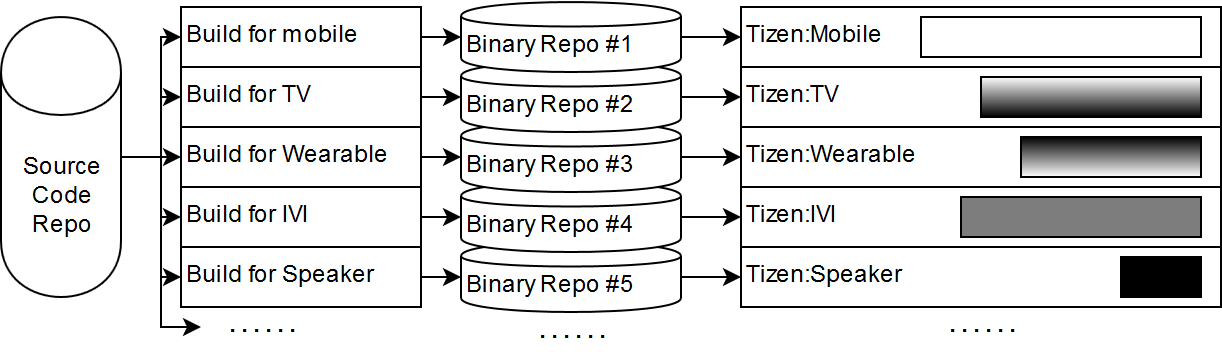
\includegraphics[width=0.95\columnwidth]{figures/TizenInfraBefore.png}
  
  \vspace{0.1cm}
  
  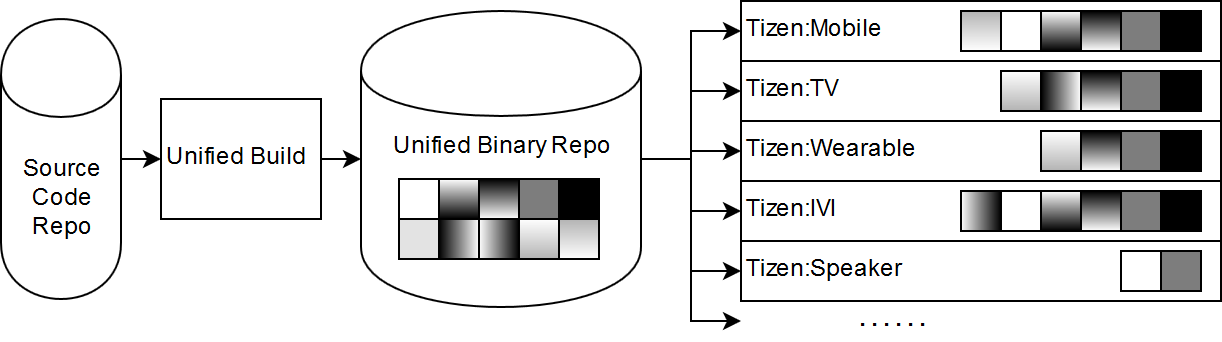
\includegraphics[width=0.95\columnwidth]{figures/TizenInfraAfter.png}
\caption{The infrastructure before and after the work.}
\label{FIG_TZN_BR_INF}
\end{figure}

Fig.~\ref{FIG_TZN_BR_INF} shows how the overall Tizen build, release, and deployment infrastructures before and after this work;
the top shows the infrastructure before this work and the bottom shows that after this work.
Before this work, adding another device type has required to multiply the build workload while it does not after this work.
In other words, adding another device type now only requires to define a new recipe with the given building blocks, which does not increase the workload visibly to the infrastructure or the developers, which requires just a few man-hour for each additional device type.
Note that with the new Tizen prototypes, autonomous driving systems and on-device AI devices, Tizen platform developers have even not been required to know the existence.


\begin{figure}
\centering
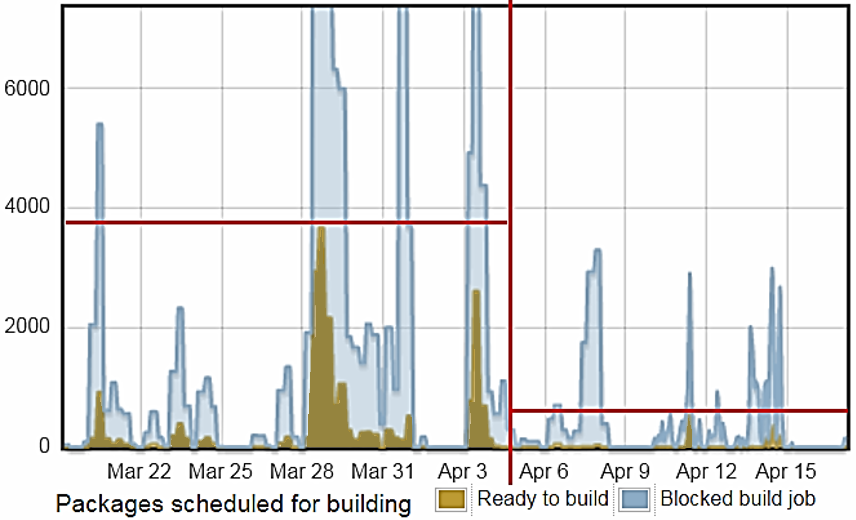
\includegraphics[width=0.95\columnwidth]{figures/tizen_build_obs_buildqueue_4wks_colored.png}
\caption{Build server task queue status in Mar-Apr, 2017}
\label{FIG_OBS_TASKQUEUE}
\end{figure}

Fig. \ref{FIG_OBS_TASKQUEUE} shows the build task workload by describing the waiting task queue lengths.
The dark khaki lines, ``Ready to build``, show the number of packages ready to be built and waiting for resource allocations.
The light blue lines, ``Blocked build job``, show the number of packages to be built, but not ready yet; i.e., even if there are resources available, we cannot build them.
We have migrated to Tizen:Unified from per-profile builds on Apr 4, which is denoted by vertical line in the middle of the figure.
Note that at this stage, Tizen 4.0 had been still in progress and Tizen 3.0 projects (per-profile basis) had been being built as well as Tizen 4.0 projects.


\begin{figure*}
\centering
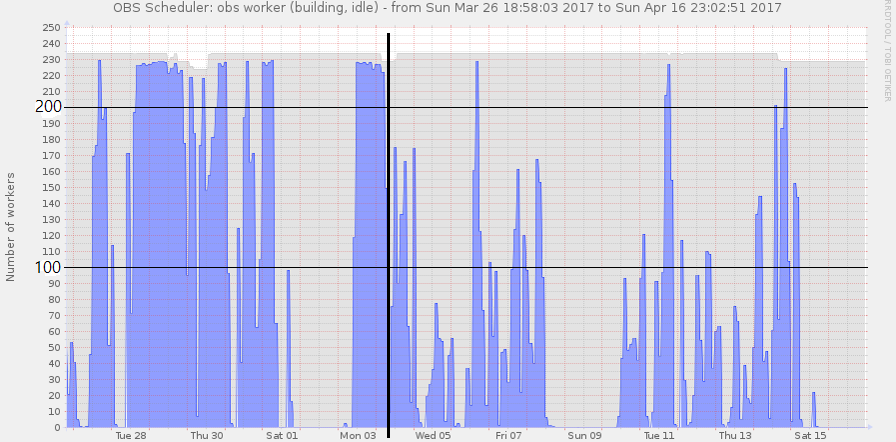
\includegraphics[width=0.90\textwidth,height=5cm]{figures/tizen_build_obs_munin.png}
\caption{Number of busy build servers in Mar-Apr, 2017. Tizen:Unified is applied at the vertical line.}
\label{FIG_OBS_MUNIN}
\end{figure*}

As we can see in Fig.~\ref{FIG_OBS_TASKQUEUE}, the peak queue length has been decreased dramatically from several thousands to less than a thousand.
Normally, the queue length has been reduced to less than dozens or zero from hundreds in typical business hours.


Fig.~\ref{FIG_OBS_MUNIN} shows the number of busy build servers.
We can again see the dramatic reduces of workloads after applying Tizen:Unified to the build system.
After Tizen:Unified is applied, developers usually no longer experience any delays in work queues; in most cases, there have been available build servers waiting for developers! This increases the productivity of developers greatly by allowing developers to get the build and integration results ready for test deployment in shorter time (within an hour, not a day).


With Tizen:Configurability, enabled by Tizen:Unified, Tizen team has started IoT projects (\url{https://wiki.tizen.org/Tizen_IoT}) along with CraftRoom~\cite{5CraftroomURL}.
Further utilizing Tizen:Unified and Tizen:Configurability, a few developers provide continuous integration and deployment services along with software platforms, one for an autonomous driving system and another for on-device AI systems as well, which is named as TAOS.
TAOS is continuously releasing its software platform binaries for both projects with frequent changes in its configurations or creations with new hardware sets and software requirements.


Without the results of Tizen:Configurability, the required build task workload and the complexity of choosing individual packages would have required far more man-month to support the two projects.
We have two members related with TAOS support and most of their workload is due to provide guides to other developers, to implement supplementary developmental tools (profilers and emulators), or to port external software packages for other developers, not on configuring and test-building software platforms.
Note that in the old days, we had needed several experts for such tasks.


